\section{\textsc{Gurkensalat}}

\subsection*{Zutaten für 2 Portionen:}

\begin{tabular}{p{7.5cm} p{7.5cm}}
	& \\
	\sfrac{1}{2} Gurke & 2EL Olivenöl \\
	1EL Essig & 1TL Zucker \\
	\multicolumn{2}{l}{Salz, Pfeffer, Dill nach Geschmack}
\end{tabular}

\subsection*{Serviervorschlag:}

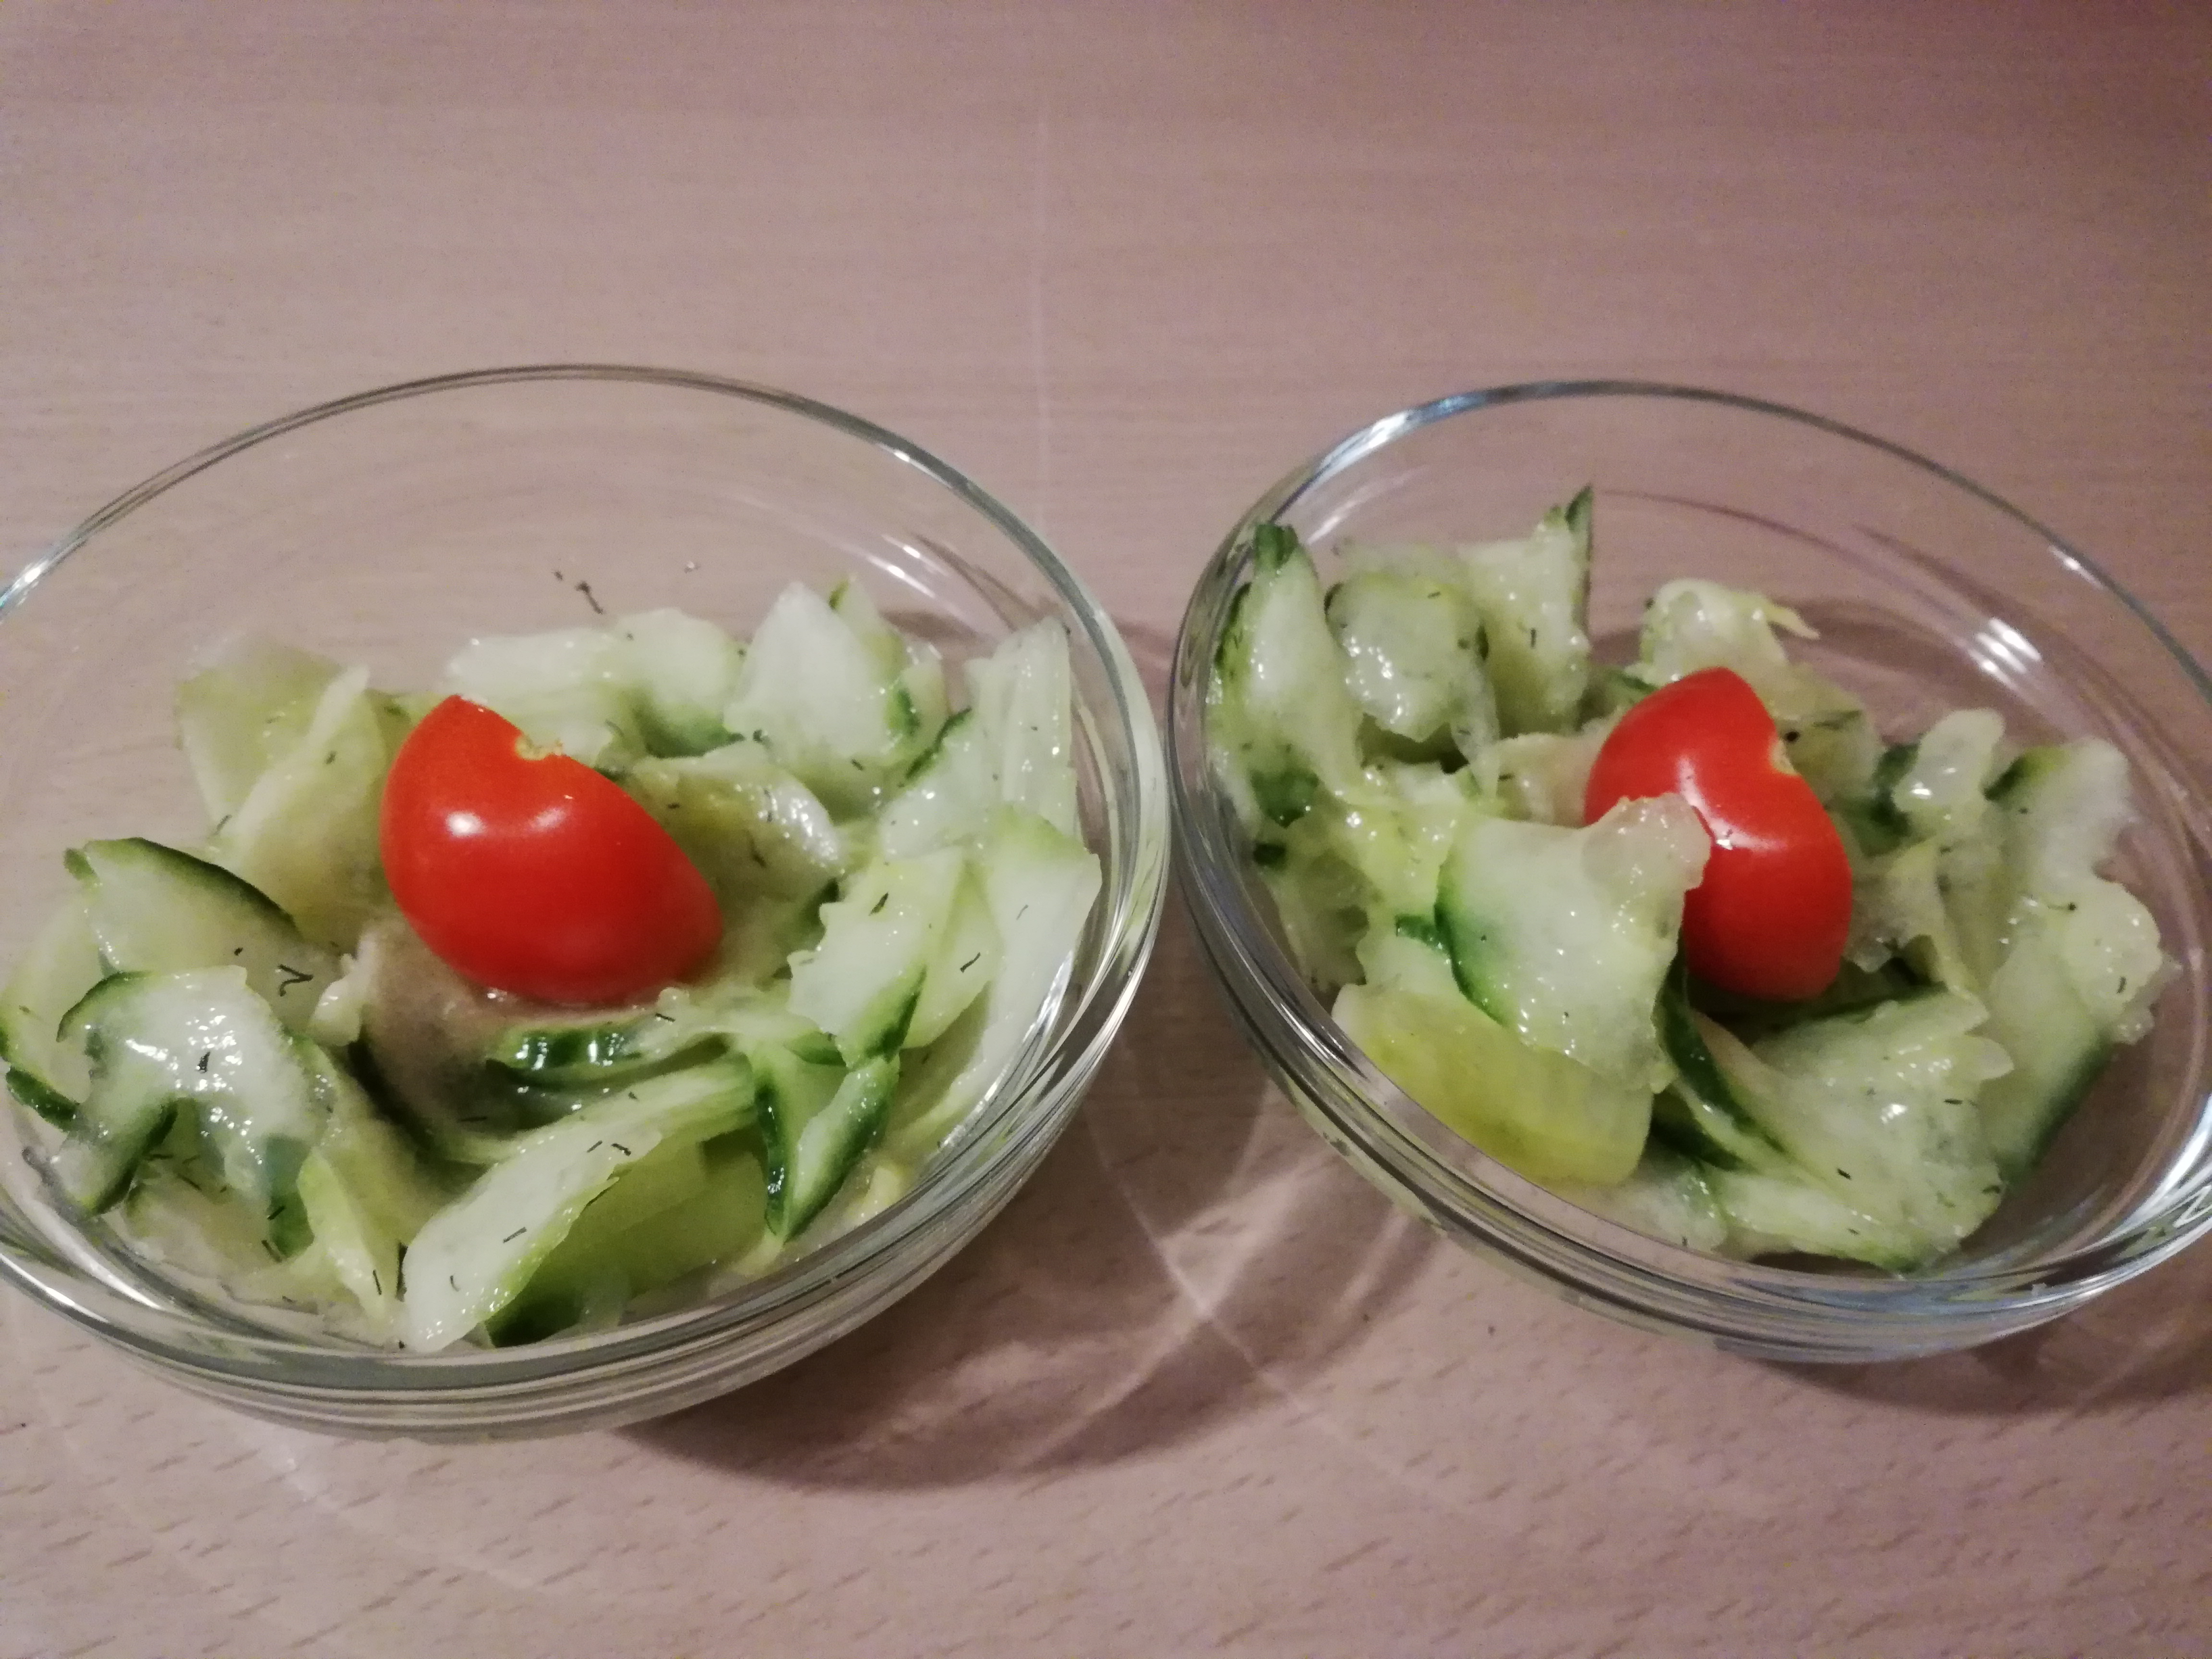
\includegraphics[width=\textwidth]{img/gurkensalat/gurkensalat_fertig.jpg} \cite{gurkensalat}

\subsection*{So geht's:}

\begin{tabular}{p{15cm}}
	\\
	Die halbe Gurke mit einem Sparschäler teilweise schälen.\\
	So entsteht ein Farbtupfer im fertigen Salat.\\
	Die Gewürze und Öle hinzufügen und alles für etwa 2h ziehen lassen.
\end{tabular}